\documentclass{beamer}
% \usepackage{animate}
\usepackage{multimedia}
\usepackage[english,russian]{babel}

\usepackage{pgfpages}
\setbeameroption{show notes on second screen}
%https://tug.ctan.org/macros/latex/contrib/beamer/doc/beameruserguide.pdf

\usepackage[T2A]{fontenc}
\usepackage[utf8]{inputenc}

\setbeamertemplate{caption}[numbered]

\usetheme{CambridgeUS}
\usecolortheme{dolphin}


\title[Мониторы]{Мониторы}
\author[Быковских Д.А.]{Быковских Дмитрий Александрович}
\date{09.11.2024}

\begin{document}
	\begin{frame}
		\titlepage
	\end{frame}

	\begin{frame}{Введение}{Первый монитор}
		
		\begin{figure}
			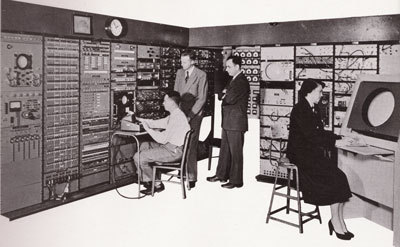
\includegraphics[width=0.47\textwidth]{images/Whirlwind-display.jpg}
			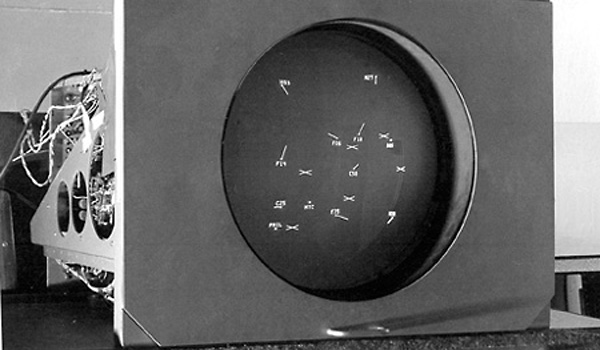
\includegraphics[width=0.5\textwidth]{images/Whirlwind-display-2.jpg}
			\caption {\href{https://www.chipsetc.com/mit-lincoln-laboratory.html}{MIT's Whirlwind 1: аппаратно-программный комплекс, 1951 г. (слева); дисплей отображающий позиций воздушные судна, 1953 г. (справа)}}
		\end{figure}


		\note{
			Первый в истории монитор появился в 1951 году и использовался в компьютере Whirlwind I (Вихрь), созданном в Массачусетском технологическом институте (MIT). 
			
			Примечания. 
			
			1. Мотивация. Для отображения информации использовалась бумага. Прорыв заключался в том, что изменения можно было увидеть в реальном времени.
			
			2. Назначение. Для научных исследований, а также военных нужд (как часть тренажеров пилотов или как радар).
			
			3. Физические размеры. Монитор был большим и громоздким по сравнению с современными, поскольку использовалась электронно-лучевая трубка.

			% https://en.wikipedia.org/wiki/Cathode-ray_tube
			
			Некоторые характеристики монитора Whirlwind I:

			% Тип матрицы: 
			\begin{itemize}
				\item 
				CRT (Cathode-Ray Tube) или ЭЛТ (электронно-лучевая трубка)
				\item
				Монохромное изображение (черно-белое изображения)
			\end{itemize}
						
			
		}
	\end{frame}

	\begin{frame}{Характеристики мониторов}
		Марка/Модель (год выпуска)\\
		Характеристики дисплея \\
		Периферия \\
		Поддержка звука \\
		Энергопотребление \\
		Внешний вид \\
		Крепление \\
		Условия эксплуатации \\
		Поддержка 3D \\

		\if 0
		Характеристики мониторов
		Марка, модель, год
			Желательно известный бренд и последних годов (не старее, чем 1 года)
		Характеристики дисплея
			Плотность пикселей (ppi)
				Размер (Диагональ, широта, высота) 27, 32, широкоформатный
				Разрешение FHD, QHD, 4K и др.
			Тип матрицы (производитель)
				NT / VA / IPS / OLED (покрытие, защита глаз)
					FAST IPS, Flicker-free technology, Low Blue Light, Quantum Dot Color
				Частота обновления (доп технологии Adaptive-Sync technology)
				Угол обзора
				Глубина цвета (битность/разрядность)
					HDR / FRC
					Цветой охват (доп технологии Wide Color Gamut)
						sRGB
						Adobe RGB (1998)
				Подсветка ()
				Яркость 
					Максимальная (от 200 до 1000 $кд/м^2$)
					Статическая ()
				Контрастность динамическая
		Порты (HDMI 2.0, DisplayPort, HUB, USB Type-C, ThunderBolt)
		Электропитание/энергопотребление
			энергоэффективность
			расположение блока
		Размер
		Вес
		Покрытие (Цвет/ глянцевое/матовое/RGB подсветка)

		Поддержка звука
		Условия эксплуатации
		Поддержка 3D
		\fi

		\note{
		Терминология

		Экран --- поверхность, на которую выводится изображение, состоящее из пикселей.
		
		Матрица --- основа дисплея, отвечающая за формирование изображения на пиксельном уровне.
		
		Дисплей --- часть монитора, представляющая собой экран (матрицу, возможно, с подсветкой), на котором формируется изображение, а также некоторые базовые компоненты для отображения изображения, например, контроллеры и порты ввода.
		
		Монитор --- готовое устройство, которое включает в себя дисплей и другие компоненты, такие как корпус, порты, встроенные контроллеры и системы питания.
		}

	\end{frame}

	% \begin{frame}{Марка/Модель}
	% 	Марка (Производитель)
		
	% 	Модель
		
	% 	\ Известность (цена/качество)\\

	% 	Год
		
	% 	 \ Желательно известный бренд и последних годов 
	% 	%  (не старее, чем 1 года)
	% \end{frame}

	\begin{frame}{PPI (Pixels Per Inch)}
		PPI (Pixels Per Inch, число пикселей на дюйм) --- показатель плотности пикселей на экране, который указывает, сколько пикселей помещается в одном дюйме экрана. 
		\[
		PPI = \frac{\sqrt{(\text{ширина}^2 + \text{высота}^2)}}{\text{диагональ}}
		\]
		Этот показатель влияет в зависимости от того, как устройство далеко расположено от глаз.\\  
		Для монитора должно быть больше 90 PPI,\\ а для смартфона --- больше 350 PPI.

		{\footnotesize
		Примеры. \\
		% Монитор 24" Full HD (1920 x 1080 пикселей) имеет 91.79 PPI\\
		Монитор 27" Full HD (1920 x 1080 пикселей) имеет 81.59 PPI\\
		Монитор 27" 1440p (2560 x 1440 пикселей) имеет 108.79 PPI\\
		Монитор 32" 4K (3840 x 2160 пикселей) имеет 137.68 PPI\\
		Samsung Galaxy S21 (6.2 дюйма, 2400 x 1080 пикселей) имеет~424.48 PPI\\
		}
		\note{

		\begin{figure}
			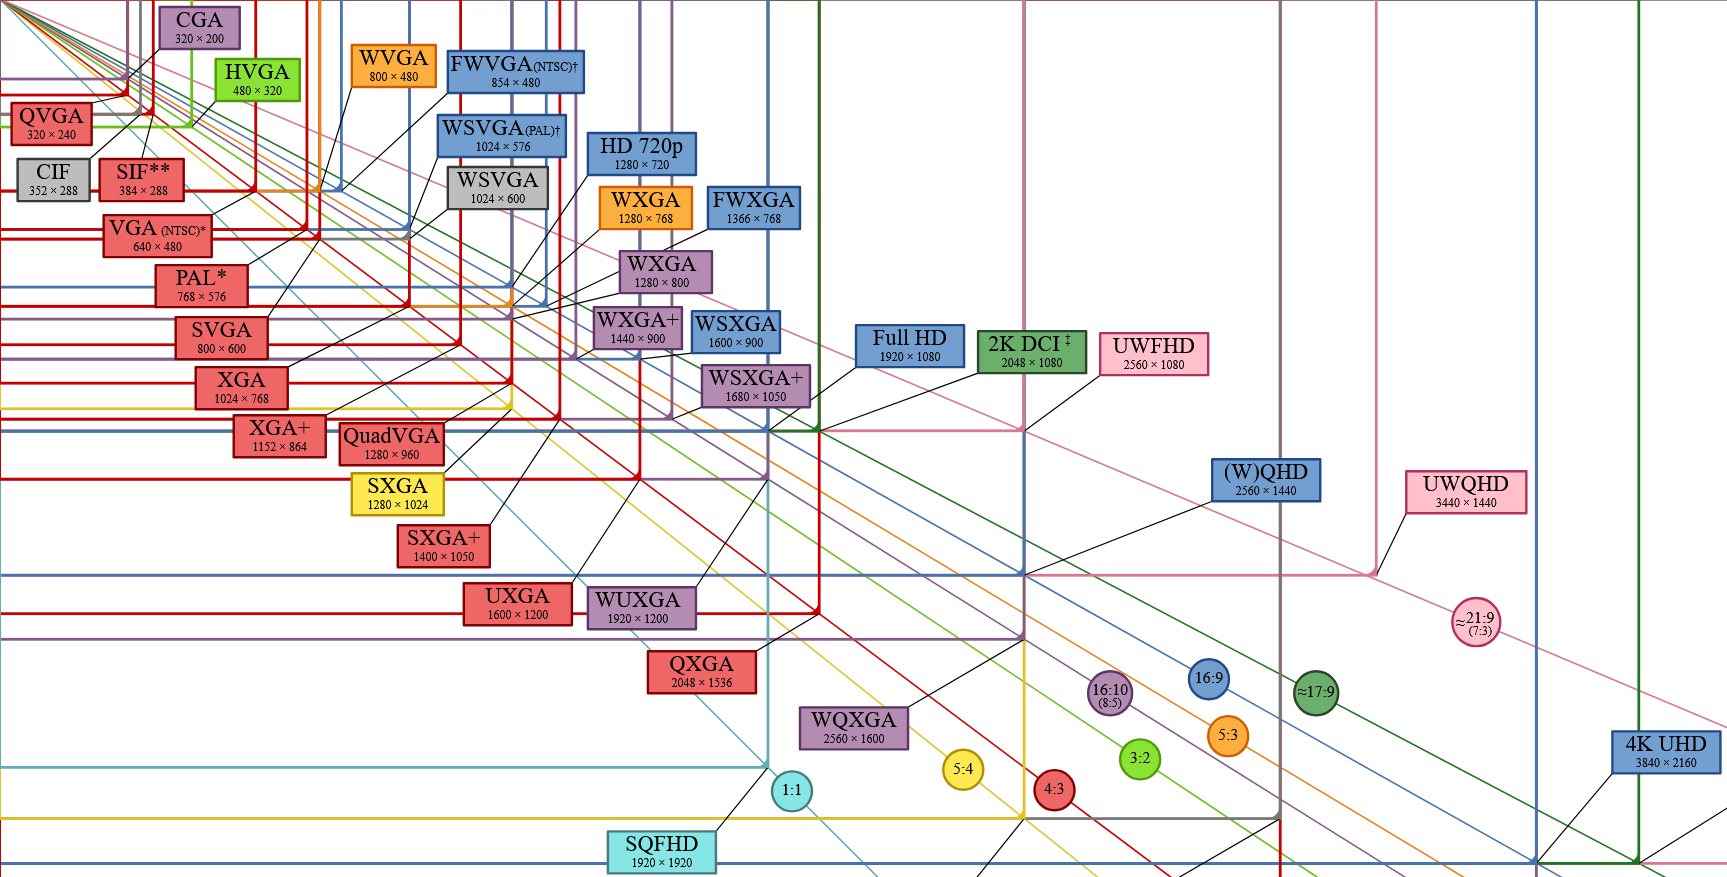
\includegraphics[width=1.0\textwidth]{images/vector-video-standards.png}
			\caption {\href{https://upload.wikimedia.org/wikipedia/commons/0/0c/Vector_Video_Standards8.svg}{Форматы разрешения экранов}}
		\end{figure}
			% Диагональ --- расстояние от одного угла экрана до противоположного, измеренное по диагонали. Это обычно указанный размер экрана (например, 27 дюймов). При этом важно помнить, что диагональ не указывает точные размеры ширины и высоты экрана.

			% Ширина и высота --- физические размеры экрана, которые зависят от разрешения и соотношения сторон. Ширина и высота также влияют на восприятие изображения и удобство работы, особенно при многозадачности или для игр.
	
			% Разрешение экрана --- количество пикселей по горизонтали и вертикали, которое формирует изображение. Чем выше разрешение, тем больше пикселей отображается на экране, что влияет на четкость изображения.
			% https://post.naver.com/viewer/postView.nhn?volumeNo=6860922&memberNo=36047368
			% https://en.wikipedia.org/wiki/Display_resolution_standards#/media/File:Vector_Video_Standards8.svg
		}
		
	\end{frame}

	\begin{frame}{Частота обновления экрана (Refresh Rate)}
		Частота обновления экрана $f$ (Гц) --- параметр, определяющий, сколько раз за одну секунду изображение на экране обновляется.

		\begin{figure}
			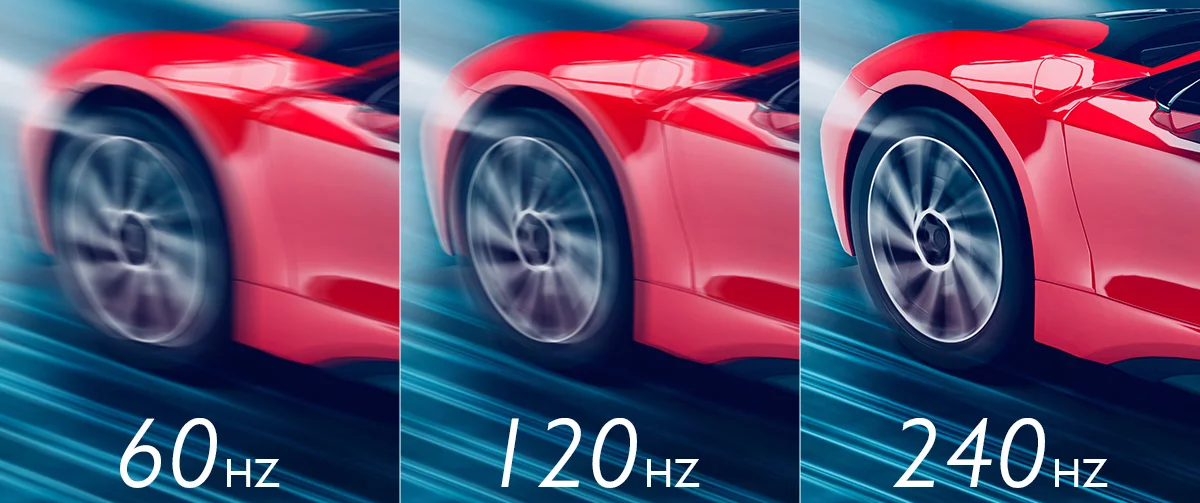
\includegraphics[width=0.55\textwidth]{images/refresh-rate.png}
			\caption {\href{https://www.benq.com/ru-ru/knowledge-center/knowledge/gaming-projector-high-refresh-rates.html}{Четкость изображения в зависимости от частоты обновления экрана}}
		\end{figure}

		% Обратная величина --- количество кадров в секунду.

		\footnotesize
		FPS (Frequency per seconds или число кадров в секунду) --- количество кадров в секунду, которое успевает отрисовать видеокарта для конкретного приложения. 
		Если частота обновления экрана f и FPS совпадают, изображение выглядит плавным. 
		Когда FPS выше частоты обновления экрана f, монитор не может отобразить все кадры, и в этом случае могут появляться артефакты, например, разрывы изображения.
		
		\note{
			{
				\footnotesize
				Пример расчета времени отклика для монитора с частотой 240 Гц.\\ $ t = 1 / 240\text{Гц} = 4.1(6)$ мс
			}
			
			Если кадры не синхронизированы, максимальная задержка $t_{max}$ отображения может достигать половины периода обновления экрана. 
			\[
				t_{max} = \frac{T}{2} = \frac{1}{2f}
				,
			\]
			где 
			$T$ --- период, 
			$f$ --- частота.


			\footnotesize
			Чтобы избежать этих проблем, можно использовать технологии синхронизации:
			
			\begin{itemize}
				\item 
				V-Sync. 
				Синхронизирует FPS и частоту обновления экрана, предотвращая разрывы изображения.
				\item
				Adaptive Sync. 
				Динамически подстраивает частоту обновления под FPS для плавного изображения.
				\item
				G-Sync (NVIDIA) и FreeSync (AMD). 
				Технологии для игровых мониторов, которые синхронизируют FPS с частотой обновления.
			\end{itemize}
			
			% Более высокая частота обновления обеспечивает более плавное движение, что особенно заметно в динамичных сценах, таких как игры, спортивные передачи и анимации.
			
		}

	\end{frame}
	
	\begin{frame}{Яркость и контрастность экрана}

		Яркость экрана --- мера интенсивности света, излучаемого экраном, и обычно выражается в нитах (nit, cd/m$^2$ или кд/м$^2$). \\
		
		{\footnotesize
			Яркость можно померить с помощью люксометра, направленный строго перпендикулярно экрану на расстоянии 1 метра, т.е. измерив световой поток в люменах и разделив на косинус угла получим канделы (кд), а площадь экрана можно вычислить исходя из его размера.
			
			% Диапазон яркости: от 200 до 1000 (рекомендуемая от 300).
			Например, для офисного использования или работы в тёмной комнате экраны с яркостью около 200-300 нит будут комфортными. 
			В ярко освещённой комнате или для наружных экранов требуется статическая яркость выше 500 нит.
		}
		Контрастность обычно измеряется как отношение яркости самого светлого белого к самому темному черному.

		\[
			\text{Контрастность} = \frac{\text{Яркость белого}}{\text{Яркость черного}}
		\]

		{\footnotesize
		Например, если белый цвет на экране имеет яркость 500 кд/м$^2$ (кандел на квадратный метр), а черный --- 0,5 кд/м$^2$, то контрастность составляет 500/0.5=1000:1.
		}
		\note{
			Регулировка яркости с помощью:

			\begin{enumerate}
				\item 
				ШИМ (Широтно-Импульсная Модуляция) \\
				Яркость экрана регулируется за счет включения и выключения подсветки с высокой частотой. 
				\item 
				аналогового управления (Direct Current Dimming или DC Dimming) \\
				Регулировка яркости постоянным током, т.е. яркость на светодиодах регулируется с помощью напряжения.
				\item 
				гибридного подхода \\
				При высоких уровнях яркости используется ШИМ с высокой частотой или DC Dimming, 
				а при низких уровнях яркости применяется ШИМ с меньшей частотой. 
				
			\end{enumerate}

			
	
		}
	\end{frame}

	\begin{frame}{Регулировка яркости экрана с помощью ШИМ}
		% Pulse With Modulation|PWM 
		ШИМ (Широтно-Импульсная Модуляция) используется для управления яркостью экрана.
		Светоизлучающие диоды (LED) --- основные источники света в большинстве современных мониторов --- могут изменять свою яркость с помощью управляемой силы тока.

		\begin{figure}
			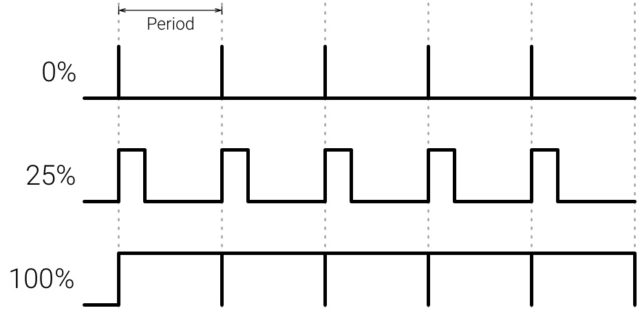
\includegraphics[width=0.75\textwidth]{images/PWM-example.jpg}
			\caption {\href{https://habr.com/ru/companies/droider/articles/519746/}{Яркость пикселя в зависимости от длительности импульса}}
		\end{figure}

		\note{
		ШИМ нужен для контроля яркости светодиодов, он управляет длительностью импульсов электрического тока. Длинный импульс --- светодиод светится ярко, а если короче --- тусклее.

		ШИМ обеспечивает плавный переход между яркими и темными областями изображения на экране. Также модуляция позволяет снизить энергопотребление, поскольку длительность импульсов можно регулировать, чтобы достичь оптимальной яркости с минимальным расходом энергии. 
		
		\footnotesize
		Примечания. \\
		1. Некоторые люди могут испытывать дискомфорт или напряжение в глазах при длительном использовании мониторов с ШИМ из-за мерцания экрана.\\
		2. Пульсация освещенности свыше 300 Гц не оказывает влияния на общую и зрительную работоспособность. ГОСТ Р 54945-2012
		
		}
	\end{frame}


	\begin{frame}{Глубина цвета}
		Глубина (битность) цвета (Color Depth) --- количество битов, которые используются для представления оттенков цвета для каждого субпикселя на экране.

		{\footnotesize
		Примеры
		\begin{itemize}
			\item 
			8-битная глубина цвета позволяет отображать 16.7 миллионов цветов (256x256x256).
			\item 
			10-битная глубина цвета дает палитру в 1.07 миллиарда цветов.
		\end{itemize}
		}

		Цветовой охват (Color Gamut) --- диапазон цветов, которые экран может воспроизводить.
		Обычно измеряется в процентах в зависимости от цветового охвата.

		{\footnotesize
		Известные цветовые охваты, используемые для сравнения, sRGB, Adobe RGB (1998), Wide Color Gamut (WCG), делящийся на DCI-P3 и Rec. 2020 (BT.2020), и др.
		}

		HDR (High Dynamic Range) --- технология, увеличивающая диапазон яркости и контрастности изображения. 

		
		\note {

			FRC (Frame Rate Control) --- технология, имитирующая более высокую битность цвета на дисплеях с ограниченной глубиной цвета. 
			
			\footnotesize
			Примеры.\\
			(FRC) 
			8-битная панель может использовать FRC для имитации 10-битного цвета, чередуя быстро отображаемые оттенки для создания промежуточных цветов. 
			Это помогает снизить полосы на градиентах, делая изображение более плавным.

			(Яркость) 
			Когда говорят о дисплее с яркостью 400 нит, обычно имеется в виду статическая яркость, то есть уровень, который экран может поддерживать постоянно. 
			\\ Если этот экран поддерживает HDR, его пиковая яркость может составлять 600-1000 нит.
			Но режим работы будет кратковременным, чтобы избежать перегрева и снижения долговечности светодиодов.

			% sRGB --- стандартный цветовой охват для веб-графики и большинства приложений. Этот охват был разработан совместно Hewlett-Packard и Microsoft в 1996 году и охватывает около 35\% всех видимых цветов, но обеспечивает совместимость с большинством устройств. Обычно используется в недорогих мониторах и устройствах, предназначенных для потребительского сегмента.
		}
		
	
	\end{frame}

	\begin{frame}{Типы матриц дипслея}
		Категории

		LCD (Liquid Crystal Display) или ЖК (жидко-кристаллический) дисплей \\
		LED (Light-Emitting Diode) дисплей \\
		OLED (Organic Light-Emitting Diode) дисплей \\

		\begin{figure}
			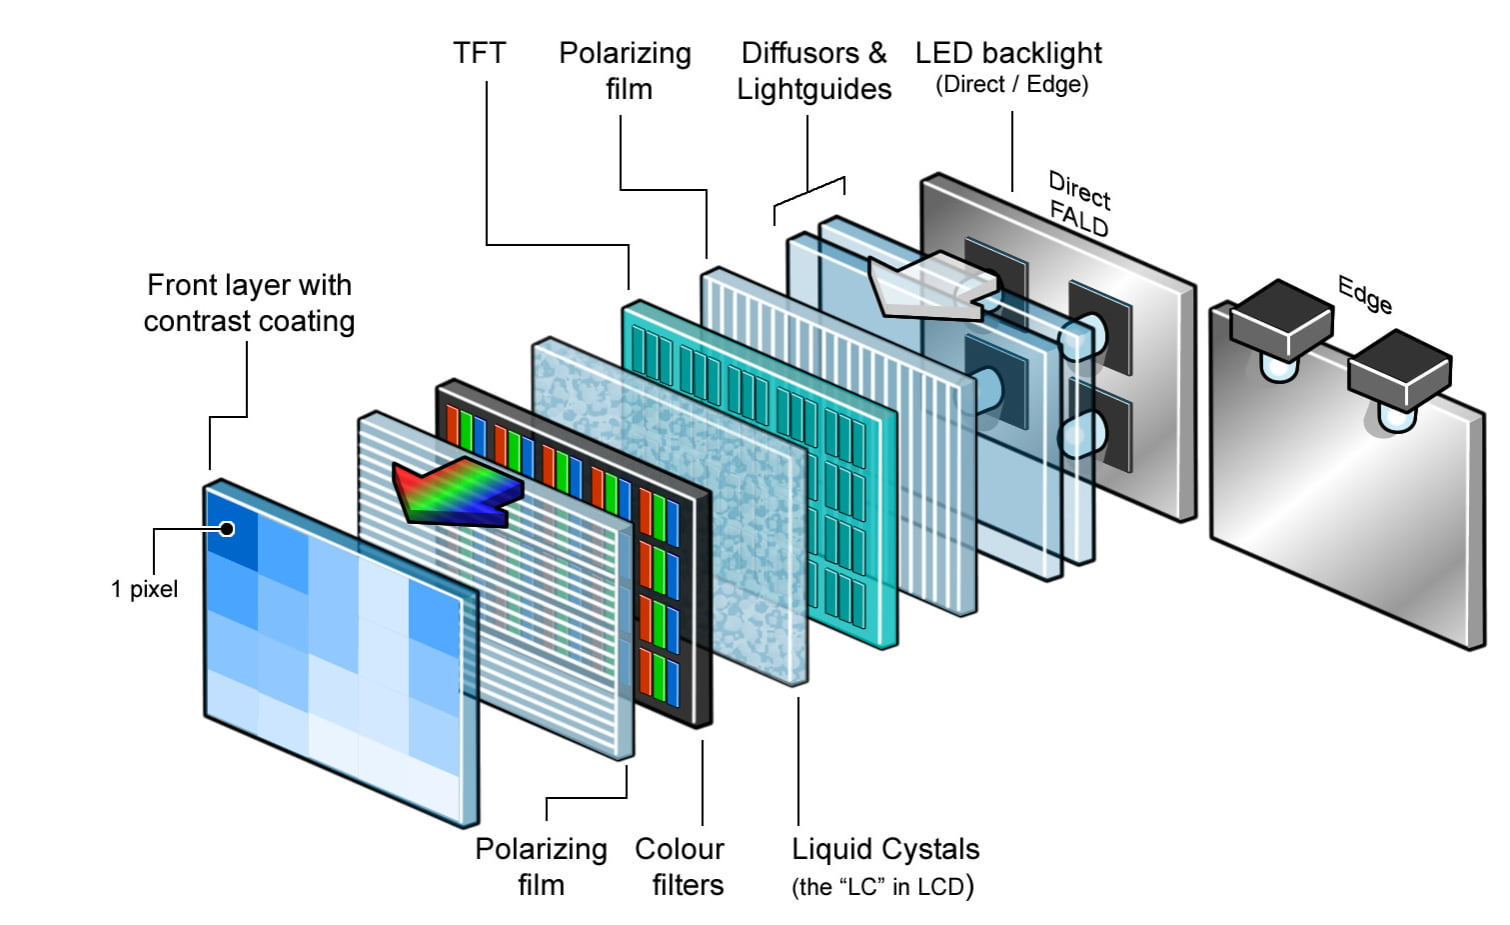
\includegraphics[width=0.45\textwidth]{images/LCD.jpg}
			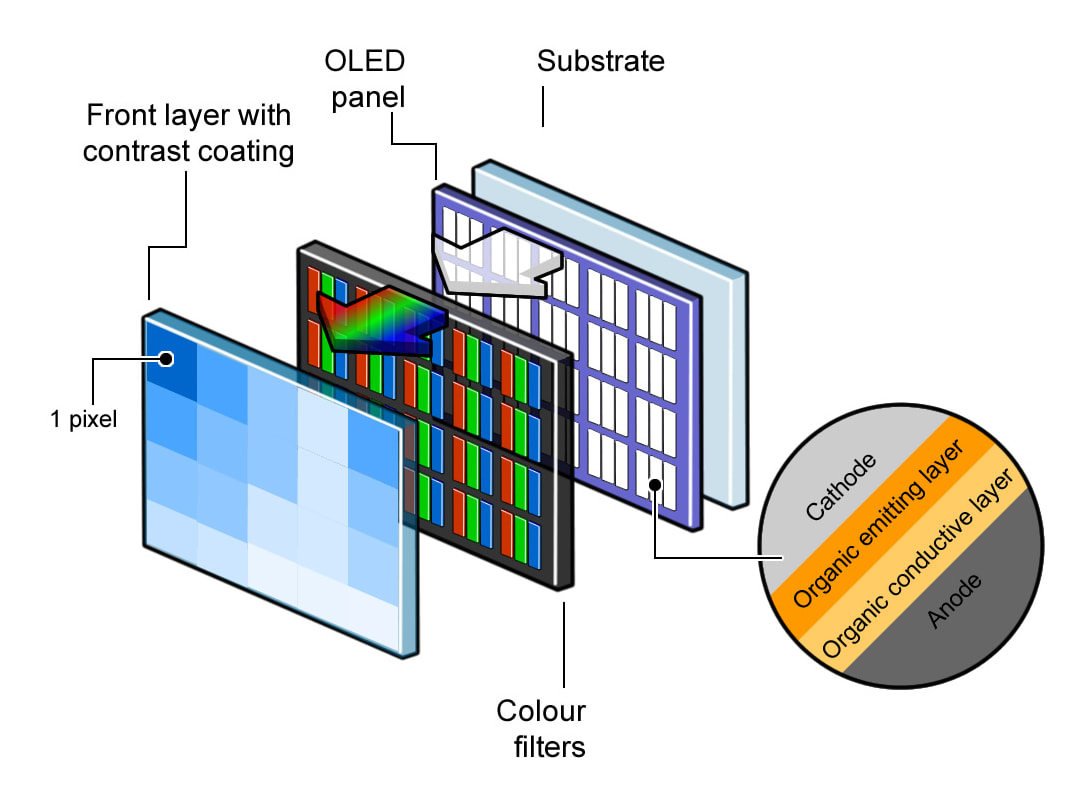
\includegraphics[width=0.45\textwidth]{images/OLED.jpg}
			\caption {\href{www.flatpanels.dk}{Матрицы диплея: LCD (слева); OLED (справа)}}
		\end{figure}

		\note{
			\footnotesize

			LCD (Liquid Crystal Display) или ЖК (жидкокристаллические) дисплеи работают на основе жидких кристаллов, которые не светятся самостоятельно, поэтому используется LED(Light-Emitting Diode) подсветка.

			Эти кристаллы размещаются между двумя слоями стекла. При подаче электрического напряжения они меняют свою ориентацию, позволяя пропускать свет или блокировать его частично, создавая изображение.

			Цветные фильтры. Каждый пиксель состоит из трех субпикселей --- красного, зеленого и синего. Изменяя степень пропускания света через каждый из субпикселей, дисплей создает разные цвета.

			\vspace{0.15cm}
			LED для подсветки ЖК-дисплеев. Светодиоды в таких дисплеях размещены позади ЖК-матрицы и служат источником света. LED-подсветка бывает боковой (edge-lit) или распределенной по задней поверхности (full-array), где светодиоды равномерно освещают ЖК-панель.

			\vspace{0.15cm}
			В OLED-дисплеях каждый пиксель состоит из органических соединений, которые светятся сами по себе при прохождении через них электрического тока. Это устраняет необходимость в дополнительной подсветке.
			% Светоизлучающие диоды (LED) --- основные источники света в большинстве современных мониторов --- могут изменять свою яркость с помощью управляемой силы тока.
		}

	\end{frame}

	\begin{frame}{Приницип работы LCD}
		

		\begin{figure}
			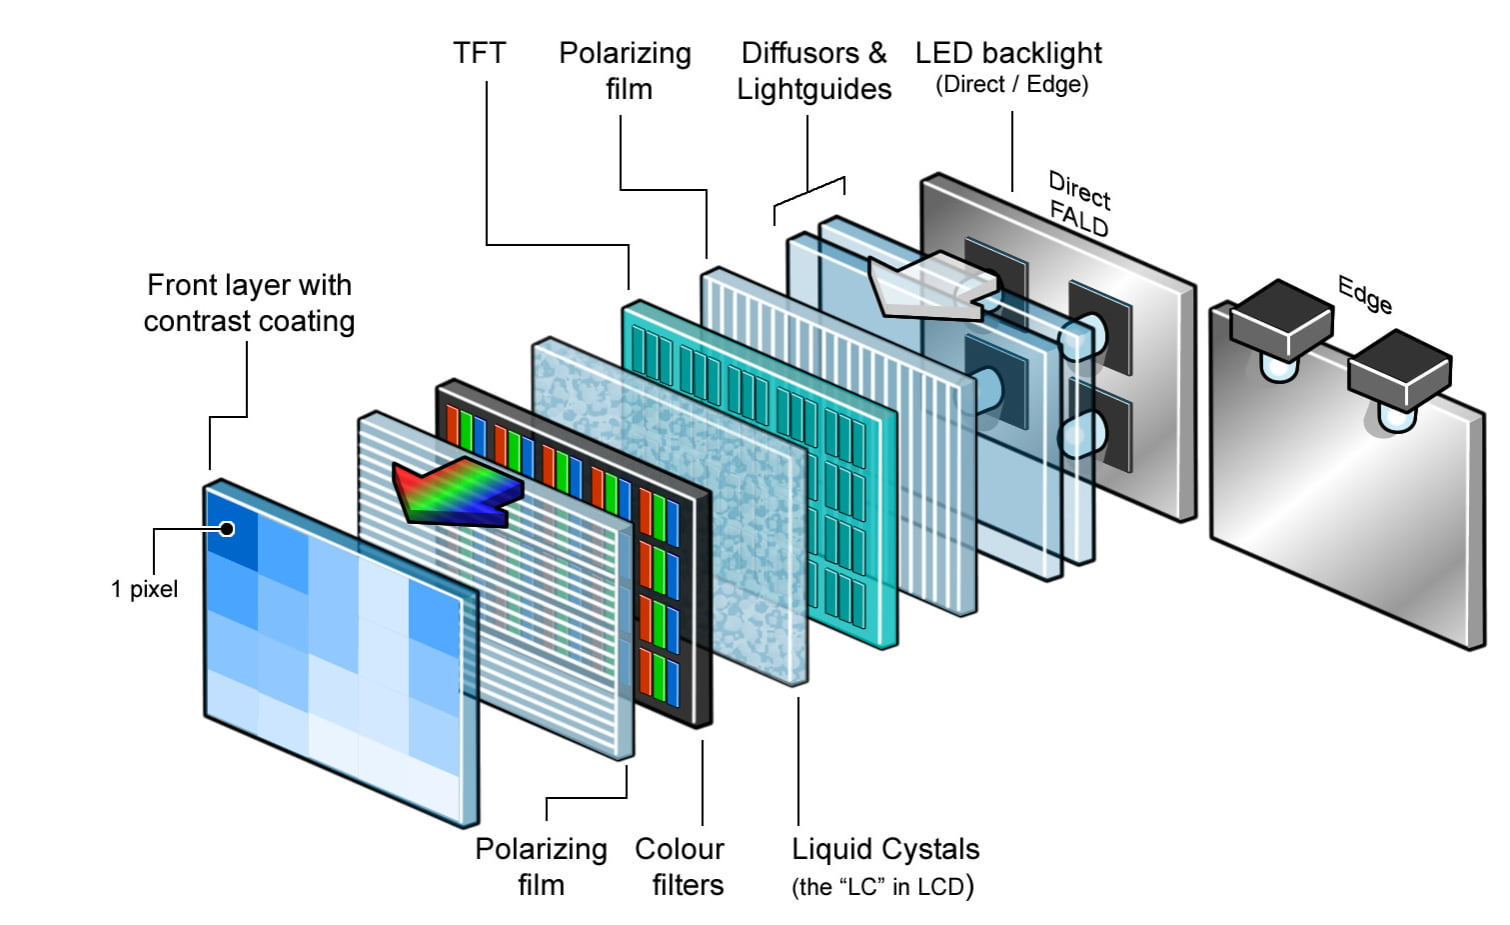
\includegraphics[width=0.85\textwidth]{images/LCD.jpg}
			\caption {\href{www.flatpanels.dk}{Принцип работы LCD}}
		\end{figure}

		\note{
			% \footnotesize
			\scriptsize

			\textbf{LED Backlight [Direct / Edge] (LED подсветка)} \\
			Источник света для подсветки ЖК-слоя. Использует светодиоды, которые могут быть расположены на задней стенке или по бокам.
			
			\textbf{Diffusors & Lightguides (Диффузоры и световоды)} \\
			Часть подсветки, отвечающая за равномерное распределение света от источников (LED). Диффузоры смягчают свет, а световоды направляют дальше.

			\textbf{Polarizing Films (Поляризационные плёнки)} \\
			Преобразуют неполяризованный свет от подсветки в поляризованный за счет ориентации.
			% ЖК-дисплей содержит два поляризационных фильтра --- один перед и один за слоем жидких кристаллов. Поляризационные фильтры ограничивают направление прохождения света. В обычных условиях свет, проходя через первый фильтр, не может пройти через второй, так как кристаллы направлены перпендикулярно. Однако, когда электрическое поле воздействует на жидкие кристаллы, они меняют ориентацию, изменяя поляризацию света и позволяя ему пройти через второй фильтр.
			
			\textbf{Liquid Crystals (Жидкие кристаллы)} \\
			Жидкие кристаллы представляют собой особое состояние вещества, которое сочетает свойства как жидкостей, так и твердых кристаллов. 
			Эти кристаллы могут изменять свою ориентацию под воздействием электрического поля, что позволяет контролировать, как свет проходит через них.
			Жидкие кристаллы расположены между стеклянными пластинами с электродами, создающие поле.
			
			\textbf{Thin-Film Transistor или TFT (Тонкоплёночный транзистор)} \\
			Каждому пикселю соответствует один транзистор, который регулирует подачу электрического сигнала.
			
			\textbf{Front Layer with Contrast Coating (Верхний слой с контрастным покрытием)} \\
			Внешний слой дисплея, который включает антибликовое (AR) или антиотражающее покрытие, а также защитное стекло или плёнку.
	

		}

	\end{frame}

	\begin{frame}{Типы LCD}
		\footnotesize
		Категории

		TN (Twisted Nematic) \\
		VA (Vertical Alignment) \\
		IPS (In-Plane Switching) \\

		\begin{figure}
			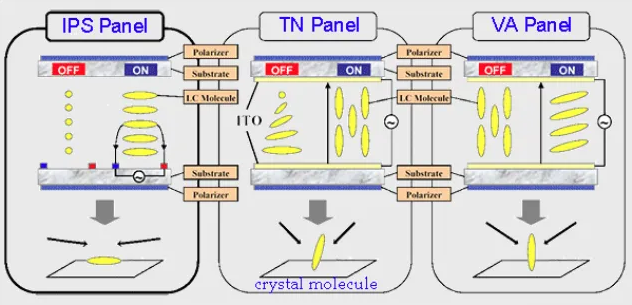
\includegraphics[width=0.85\textwidth]{images/LCD-types.png}
			\caption {\href{https://4k-monitor.ru/about/howto/tipy_matric_monitorov/}{Типы матриц: IPS (слева); TN; VA (справа)}}
		\end{figure}

		\note{
			% \footnotesize
			\scriptsize
			Виды\\
			\textbf{ TN (Twisted Nematic или скрученный нематик)} \\
			В TN матрицах кристаллы при включении «скручиваются» между поляризаторами, что позволяет изменять их ориентацию и регулировать прохождение света.\\
			Примечание. Нематик --- один из типов жидких кристаллов, которые представляют собой вещества с упорядоченной ориентацией молекул.\\
			% 6 bit + FRC
			\textbf{ VA (Vertical Alignment или вертикальное выравнивание)} \\
			В VA матрицах кристаллы выстраиваются вертикально, что улучшает контрастность, так как в отключенном состоянии они блокируют свет лучше.\\
			
		
			\textbf{ IPS (In-Plane Switching или переключение в плоскости)} \\
			В IPS матрицах кристаллы расположены параллельно экрану, что позволяет более точно управлять ими и обеспечивать широкие углы обзора.\\
			Примечание. Технология \textbf{FAST IPS} с быстрым временем отклика (1-2 мс.)

			\if 0
			\begin{itemize}
				\item 
				TN (Twisted Nematic или скрученный нематик) \\
				В TN матрицах кристаллы при включении «скручиваются» между поляризаторами, что позволяет изменять их ориентацию и регулировать прохождение света.\\
				Примечание. \\
				Нематик --- один из типов жидких кристаллов, которые представляют собой вещества с упорядоченной ориентацией молекул.
				% 6 bit + FRC
				\item 
				VA (Vertical Alignment или вертикальное выравнивание) \\
				В VA матрицах кристаллы выстраиваются вертикально, что улучшает контрастность, так как в отключенном состоянии они блокируют свет лучше.
				\item 
				IPS (In-Plane Switching или переключение в плоскости) \\
				В IPS матрицах кристаллы расположены параллельно экрану, что позволяет более точно управлять ими и обеспечивать широкие углы обзора.

			\end{itemize}
			\fi
				\vspace{0.15cm}
			Примечания связанные с LED подсветкой.\\
			1. QLED (QD-LED) подсветка Quantum Dot (Квантовые точки). Вместо традиционного фосфорного люминофора используют слой, так называемых, квантовых точек, позволяющий увеличить цветовой охват LCD матрицы и сделать цвета более насыщенными.\\
			2. Mini-LED --- подсветка, состоящая из тысяч миниатюрных светодиодов. 

		}

	\end{frame}

	\begin{frame}{OLED}
		
		\begin{figure}
			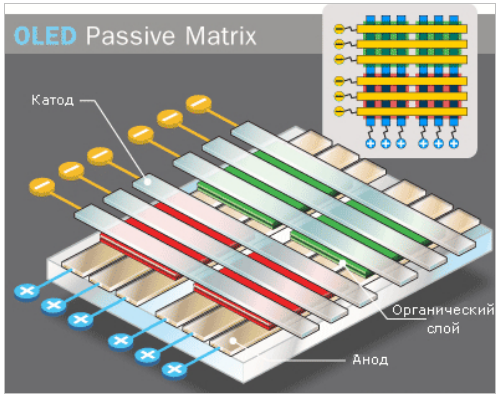
\includegraphics[width=0.49\textwidth]{images/passive-matrix-OLED.png}
			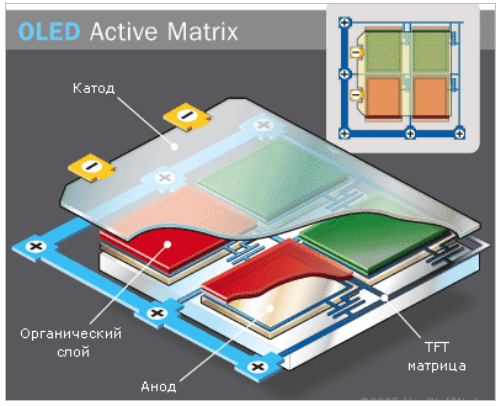
\includegraphics[width=0.48\textwidth]{images/active-matrix-OLED.png}
			\caption {\href{https://al-tm.ru/stati/monitoram/displei-na-organic-light-emitting-diode-(oled)}{OLED матрицы: PMOLED (слева); AMOLED (справа)}}
		\end{figure}
 				

		\note{
			\scriptsize
			Принцип работы основан на электролюминесценции\\

			OLED-дисплеи используют органические материалы, которые могут излучать свет при подаче электрического тока. 
			Эти материалы размещены в виде тонких слоев между двумя электродами.
			% Когда на эти слои подается электрическое напряжение, электроны и дырки (положительные заряды) встречаются и рекомбинируются, что вызывает эмиссию света. \\
   		% Обычно один из электродов --- анод, который прозрачен, а другой --- катод. Через анод ток подается на органические слои, где происходит выделение света.
			Один из электродов --- анод (прозрачный), а другой --- катод.
			При подаче напряжения электроны и дырки (положительные заряды) встречаются и рекомбинируются, что вызывает эмиссию света.

			% https://pikabu.ru/story/pochemu_anod_anod_a_katod_katod_prichyom_tut_metabolizm_kachkov_i_pokhod_10_000_grekov_v_anatoliyu_11229365

			\vspace{0.15cm}
			Passive-matrix OLED (PMOLED)\\
			OLED с пассивной матрицей состоит из многочисленных полосок-катодов, органических слоев и полосок-анодов.
			Место пересечения катодов и анодов - испускающие свет пиксели. 
			В зависимости от того, какой пиксель нужно "включить", на ту или иную пару катод/анод подается напряжение. 
			PMOLED несложен в производстве, однако он потребляет больше энергии, чем другие типы OLED. 
			% Лучше всего такой вариант подходит для дисплеев небольшого размера - в мобильных телефонах, КПК и MP3-плеерах. Впрочем, даже PMOLED потребляют меньше энергии, чем LCD сопоставимого размера.

			\vspace{0.15cm}
			Active-matrix OLED (AMOLED)\\
			OLED с активной матрицей использует лишь одну пару катод/анод (в этом случае применяются не полоски, а настоящие панели). 
			Кроме того, анод имеет подложку из тонкопленочных транзисторов (TFT или Thin-Film Transistor), которая и «указывает», к какой области слоя подается электрический ток. 
			AMOLED потребляет меньше энергии и, поэтому, может использоваться в дисплеях большего размера. 
			%  В случае с видео - дисплеи с активной матрицей имеют лучшее время отклика. AMOLED можно применять в мониторах, телевизорах и рекламных биллбордах.

			%  Глянцевое покрытие
		}

			
	\end{frame}

% 	\begin{frame}{Технологии, разработанные для защиты зрения}

% 	Технологии, разработанные для защиты зрения:
			
% 	Flicker-Free (Отсутствие мерцания при низких уровнях яркости)
% 	%Уменьшает или полностью устраняет мерцание экрана при низких уровнях яркости, которое возникает из-за работы светодиодной подсветки на высоких частотах (PWM --- широтно-импульсная модуляция). Отсутствие мерцания снижает нагрузку на глаза и усталость, особенно при длительном использовании.

% 	Low Blue Light (Пониженное синее свечение)
% 	% Технология снижения синего света уменьшает количество излучаемого синего спектра, который может способствовать усталости глаз и нарушению сна. Этот режим снижает интенсивность синих оттенков, что более комфортно для длительного просмотра.

% 	Anti-Glare Coating (Антибликовое покрытие)
% 	% Специальное покрытие экрана помогает уменьшить блики от внешнего света, что делает изображение более четким и снижает напряжение глаз. Это особенно полезно для работы в ярко освещенных помещениях.

% 	Adaptive Brightness (Адаптивная яркость) или любая подобная технология
% 	% Адаптивная яркость корректирует уровень подсветки в зависимости от отображаемого контента, делая яркие изображения менее яркими, а темные --- наоборот. Это уменьшает резкие перепады яркости, которые могут напрягать зрение.


% 	Примечание.\\
% 	% TUV Rheinland Certification
% 	TUV Rheinland --- сертификация, подтверждающая, что монитор прошел испытания на безопасность для зрения. Сертифицированные модели обычно оснащены технологиями Flicker-Free и Low Blue Light.
% \end{frame}

	\begin{frame}{Итоговое сравнение}
		\scriptsize

		\begin{table}[h!]
			\centering
			\begin{tabular}{|p{1.2cm}|p{1.2cm}|p{1.7cm}|p{2cm}|p{1.1cm}|p{2.1cm}|}
			\hline
			\textbf{Матрица} & \textbf{Время отклика} & \textbf{Частота обновления} & \textbf{Цветопередача} & \textbf{Угол обзора*} & \textbf{Контрастность} \\ \hline
			\textbf{TN}         & $\sim$1 мс            & До 240 Гц                   & 45--60\% sRGB          & 160$^\circ$                  & $\sim$1000:1           \\ \hline
			\textbf{VA}         & 4--6 мс               & До 240 Гц                   & 70--90\% sRGB          & 178$^\circ$                  & $\sim$3000:1 (выше)    \\ \hline
			\textbf{IPS}        & 4--5 мс               & До 144 Гц                   & 95--100\% sRGB         & 178$^\circ$                  & $\sim$1000:1           \\ \hline
			\textbf{Fast IPS}   & 1--2 мс               & До 360 Гц                   & 95--100\% sRGB         & 178$^\circ$                  & $\sim$1000:1           \\ \hline
			\textbf{OLED}       & $<$1 мс               & До 240 Гц                   & 100\% DCI-P3 / sRGB    & 178$^\circ$                  & Бесконечная**            \\ \hline
			\end{tabular}
			\caption{Сравнение технологий дисплеев}
			\label{tab:display_technologies}
			\end{table}

			\if 0
		% \begin{table}[h!]
		% 	\centering
		% 	\begin{tabular}{|p{1cm}|p{2cm}|p{1.2cm}|p{2.1cm}|p{1.8cm}|p{1.3cm}|}
		% 	\hline
		% 	\textbf{Тип матрицы} & \textbf{Контрастность} & \textbf{Углы обзора} & \textbf{Цветопередача} & \textbf{Время отклика} & \textbf{Цена} \\
		% 	\hline
		% 	TN & Низкая & Узкие & Умеренная & $\sim$1 мс & Низкая \\
		% 	\hline
		% 	VA & Высокая & Средние & Хорошая & 4--6 мс & Средняя \\
		% 	\hline
		% 	IPS & Средняя & Широкие & Отличная & 4--5 мс & Высокая \\
		% 	\hline
		% 	OLED & Бесконечная* & Широкие & Превосходная & $<$1 мс & Высокая \\
		% 	\hline
		% 	\end{tabular}
		% 	\caption{Характеристики популярных типов матриц}
		% 	\label{tab:matrix_types}
		% \end{table}
		\fi

		Примечания.\\
		Гамут sRGB --- 35\%; Гамут DCI-P3 --- 45\%\\
		*Угол обзора по вертикали и горизонтали одинаковый.\\
		**Это возможно, если устройство, например, OLED-дисплей, использует самосветящиеся пиксели, каждый из которых может быть полностью выключен для отображения черного.\\


		\note {
			Технологии, разработанные для защиты зрения
			\begin{itemize}
				\item 
				Flicker-Free (Отсутствие мерцания при низких уровнях яркости)
				%Уменьшает или полностью устраняет мерцание экрана при низких уровнях яркости, которое возникает из-за работы светодиодной подсветки на высоких частотах (PWM --- широтно-импульсная модуляция). Отсутствие мерцания снижает нагрузку на глаза и усталость, особенно при длительном использовании.
				\item 
				Low Blue Light (Пониженное синее свечение)
				% Технология снижения синего света уменьшает количество излучаемого синего спектра, который может способствовать усталости глаз и нарушению сна. Этот режим снижает интенсивность синих оттенков, что более комфортно для длительного просмотра.
				\item 
				Anti-Glare Coating (Антибликовое покрытие)
				% Специальное покрытие экрана помогает уменьшить блики от внешнего света, что делает изображение более четким и снижает напряжение глаз. Это особенно полезно для работы в ярко освещенных помещениях.
				\item 
				Adaptive Brightness (Адаптивная яркость) или любая подобная технология
				% Адаптивная яркость корректирует уровень подсветки в зависимости от отображаемого контента, делая яркие изображения менее яркими, а темные --- наоборот. Это уменьшает резкие перепады яркости, которые могут напрягать зрение.
			\end{itemize}
			
			\footnotesize
			Примечание.\\
			% TUV Rheinland Certification
			TUV Rheinland --- сертификация международным концерном, подтверждающая, что монитор прошел испытания на безопасность для зрения. 
			Сертифицированные модели обычно оснащены технологиями Flicker-Free и Low Blue Light.
		}

	\end{frame}



	\begin{frame}{Остальные характеристики монитора}
		\begin{itemize}
			\item 
			Энергопотребление
			\item 
			Порты (HDMI, DisplayPort (DP), ThunderBolt, HUB, USB Type-C)
			\item 
			Дизайн и внешний вид
			\begin{itemize}
				\item Размер
				\item Свойства материала (цвет, глянцевый, матовый и т.д.) 
				\item RGB подсветка
			\end{itemize}
			\item 
			Вес
			\item 
			Условия эксплуатации
			\item 
			Крепление
			\item
			Поддержка звука
		\end{itemize}
		
		\note{
			\scriptsize

			\begin{table}[h!]
				\centering
				\begin{tabular}{|c|c|c|c|}
				\hline
				\textbf{Стандарт}   & \textbf{Год выпуска} & \textbf{Максимальное разрешение}     & \textbf{Частота обновления}       \\ \hline
				\textbf{DP 1.1}     & 2008                & 2560x1600                             & 60 Гц                             \\ \hline
				\textbf{DP 1.2}     & 2010                & 3840x2160 (4K)                        & 60 Гц                             \\ \hline
				\textbf{DP 2.0}     & 2019                & 3840x2160 (4K)                        & 240 Гц (4K)                       \\ \hline
				\textbf{DP 2.0}     & 2019                & 10240x4320 (10K)                      & 60 Гц                             \\ \hline

				\textbf{HDMI 2.0}   & 2013                & 3840x2160 (4K)                        & 60 Гц                             \\ \hline
				\textbf{HDMI 2.1}   & 2017                & 3840x2160 (4K)                        & 120 Гц                            \\ \hline
				\textbf{HDMI 2.1}   & 2017                & 7680x4320 (8K)                        & 60 Гц                             \\ \hline
				\end{tabular}
				\caption{Характеристики версий DisplayPort и HDMI}
				\label{tab:dp_hdmi_versions}
			\end{table}
			
			\footnotesize
			Крепление 
			\begin{itemize}
				\item 
				Подставка монитора (с дополнительной регулировкой угла наклона и поворота)
				\item
				Совместимость с креплением VESA (использовать кронштейн)\\
			\end{itemize}
		}

	\end{frame}

	\begin{frame}{Поддержка 3D}
		
		\begin{figure}
			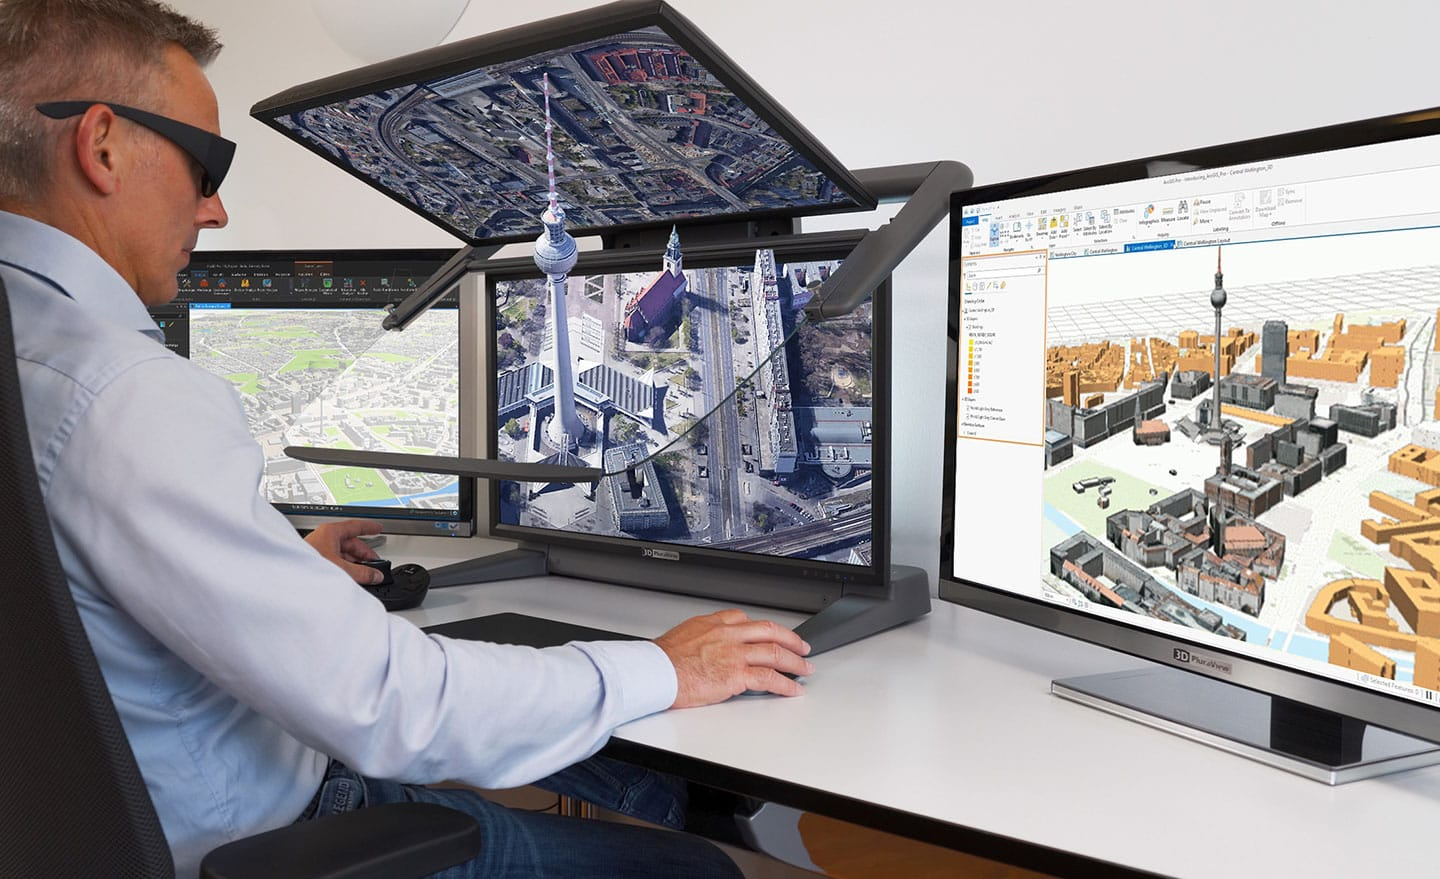
\includegraphics[width=0.8\textwidth]{images/3d-monitor.jpeg}
			\caption {\href{https://www.surveyinggroup.com/what-is-a-3d-monitor-everything-you-need-to-know-about/}{Passive 3D Stereo Monitor}}
		\end{figure}

		\note {

			Поддержка 3D в мониторах означает, что они могут отображать изображения, создающие иллюзию глубины, что позволяет зрителю видеть «объемные» изображения или видео. 
	
			Это достигается путем раздельного показа изображения для левого и правого глаза, что в мозге формирует стереоскопический эффект. 
	
			Основные технологии 3D-дисплеев включают:
			\begin{itemize}
				\item 
				Активные затворные очки. Основано на чередовании кадров. 
				% Каждый глаз видит отдельное изображение, синхронизированное с обновлением экрана с помощью очков с затворами. Такие мониторы чередуют кадры для левого и правого глаза с высокой скоростью.
				\item 
				Поляризационные очки. 
				% Экран монитора одновременно отображает два изображения с разной поляризацией, и очки разделяют изображения для левого и правого глаза. Поляризационные дисплеи, как правило, не требуют высокой частоты кадров, но могут уменьшать общее разрешение.
				\item 
				Автостереоскопические дисплеи. Специальные линзы (или параллакс-барьеры) с ограниченным углом обзора.
				% Такие мониторы не требуют очков и используют линзы или параллакс-барьеры для направления изображения в каждый глаз. Это более сложная технология, и автостереоскопические дисплеи обычно имеют ограниченные углы обзора.
			\end{itemize}
						
			\footnotesize
			Пик популярности 2010-х годов.

			Причины непопулярности.
				
				1. Ограниченный контент дорогое производство.
	
				2. Неудобство использования из-за дополнительных аксессуаров
	
				3. Усталость глаз и головная боль.

		}

	\end{frame}

	% \begin{frame}{Список источников}

	% https://www.displayspecifications.com/

	% https://4k-monitor.ru/
		
	% \end{frame}

\end{document}
